% -*- TeX:de -*-
\NeedsTeXFormat{LaTeX2e}
\documentclass[12pt,a4paper]{article}
\usepackage[german]{babel} % german text
\usepackage[DIV12]{typearea} % size of printable area
\usepackage[T1]{fontenc} % font encoding
%\usepackage[latin1]{inputenc} % most likely on Windows
\usepackage[utf8]{inputenc} % probably on Linux
\usepackage{multicol}

% PLOTTING
\usepackage{pgfplots} 
\usepackage{pgfplotstable}
\usepackage{url}
\usepackage{graphicx} % to include images
\usepackage{tikz}
\usepackage{subfigure} % for creating subfigures
\usepackage{amsmath} % a bunch of symbols
\usepackage{amssymb} % even more symbols
\usepackage{booktabs} % pretty tables
\usepackage{makecell} % multi row table heading

% a floating environment for circuits
\usepackage{float}
\usepackage{caption}

%\newfloat{circuit}{tbph}{circuits}
%\floatname{circuit}{Schaltplan}

% a floating environment for diagrams
%\newfloat{diagram}{tbph}{diagrams}
%\floatname{diagram}{Diagramm}
\pgfplotsset{compat=1.8}
\selectlanguage{german} % use german

\begin{document}

%%%%%%% DECKBLATT %%%%%%%
\thispagestyle{empty}
			\begin{center}
			\Large{Fakultät für Physik}\\
			\end{center}
\begin{verbatim}


\end{verbatim}
							%Eintrag des Wintersemesters
			\begin{center}
			\textbf{\LARGE SS 14}
			\end{center}
\begin{verbatim}


\end{verbatim}
			\begin{center}
			\textbf{\LARGE{Physikalisches Praktikum\\ für das Bachelorstudium}}
			\end{center}
\begin{verbatim}




\end{verbatim}

			\begin{center}
			\textbf{\LARGE{PROTOKOLL}}
			\end{center}
			
\begin{verbatim}

\end{verbatim}

			\begin{flushleft}
			\textbf{\Large{Experiment (Nr., Titel): PS1 - Schwingungen 1}\\
							%Experiment Nr. und Titel statt den Punkten eintragen
			\LARGE{PS1}}	
			\end{flushleft}

\begin{verbatim}

\end{verbatim}	
							%Eintragen des Abgabedatums, oder des Erstelldatums des Protokolls
			\begin{flushleft}
			\textbf{\Large{Datum:}} \Large{05.06.2014}
			\end{flushleft}
			
\begin{verbatim}
\end{verbatim}
							%Namen der Protokollschreiber
		\begin{flushleft}
			\textbf{\Large{Namen:}} \Large{Patrick Braun, Johannes Kurz}
			\end{flushleft}

\begin{verbatim}


\end{verbatim}
							%Kurstag und Gruppennummer, zb. Fr/5
			\begin{flushleft}
			\textbf{\Large{Kurstag/Gruppe:}} \Large{DO/4}
			\end{flushleft}

\begin{verbatim}

\end{verbatim}
							%Name des Betreuers, das Praktikum betreute.
			\begin{flushleft}
			\LARGE{\textbf{Betreuer:}}	\Large{Wilhelm Markowitsch}	
			\end{flushleft}

%%%%%%% DECKBLATT ENDE %%%%%%%
\pagebreak
\setlength{\columnsep}{20pt}
\begin{multicols}{2}

%%%%%%%%%%%%%%%%%%%%%%%%%%%%%%%%%%%%%%%%%%%%%%%%

%\begin{figure}[H]
%	\centering
%	\includegraphics[scale=0.35]{./data/beugung.png}
%	\caption{Beugungsmuster Einzelspalt (echtes Foto; schwarz durch weiß ersetzt)}
%	\label{fig:beugungsmuster}
%\end{figure}


%\begin{figure}[H]
%	\centering
%	\pgfplotstabletypeset[
%			columns={abstand, n},
%			col sep=&,
%			columns/abstand/.style={precision=2, zerofill, column name=\makecell{$Abstand$\\$(\pm 0.05)[mm]$} }, 
%			columns/n/.style={column name=\makecell{$n$\\$(Ordnung)$}, precision=0},
%			every head row/.style={before row=\hline,after row=\hline\hline},
%			every last row/.style={after row=\hline},
%			every first column/.style={column type/.add={|}{} },
%			every last column/.style={column type/.add={}{|} }
%			]{
%			abstand & n
%			12.9 & 1
%			24.45 & 2
%			37.40 & 3
%			49.35& 4
%			62.45 & 5
%			74.45 & 6
%			87.45 & 7
%			100.25 & 8
%			
%			}
%	\caption{Messwerte Einzelspalt}
%	\label{tab:werte_einzelspalt}
%\end{figure}


%%%%%%%%%%%%%%%%%%%%%%%%%%%%%%%%%%%%%%%%%%%%%%%%
%%%%%%%%%%%%%%%%%%%%%%%%%%%%%%%%%%%%%%%%%%%%%%%%


\section{Schwingungen 1}
In PS1 werden mechanische Oszillatoren auf ihre Eigenschaften untersucht.\\
Im Detail werden ein Drehpendel, ein gekoppeltes Pendel und die Dopplerverschiebung betrachtet. Dabei werden gedämpfte Schwingungen, auch getriebene sowie Schwebungen (Kopplung, Dopplereffekt) untersucht.
%%%%%%%%%%%%%%%%%%%%%%%%%%%%%%%%%%%%%%%%%%%%%%%%%%%%%%%%%%%%%%%%%%%%%%%
\section{Grundlagen:}
Die Bewegungsgleichung, die einen gedämpften harmonischen Oszillator beschreibt ist klassisch gegeben durch:
$$m  \ddot{x} + k \dot{x} + D x = 0$$
$m$... Masse\\
$k$... Reibungszahl\\
$D$... Federkonstante\\

\noindent Die Lösung der Gleichung für den ungedämpften (k=0) harmonischen Oszillator sind die Winkelfunktionen:
$$x(t) = A \cdot cos(\omega t + \phi)$$
Dabei ist \textbf{A} die Amplitude, \textbf{$\omega$} die Kreisfrequenz, \textbf{t} die Zeit und \textbf{$\phi$} die Phase, also die Auslenkung, mit der die Schwingung begonnen hat (zu t=0).\\
Betrachtet man nun eine gedämpfte Schwingung ergibt sich als Lösung ein zusätzlicher zeitabhängiger Dämpfungsterm: 
$$x(t) = A \cdot e^{- \delta t} \cdot cos(\omega t + \phi)$$ 
Hierbei ist $\delta$ die Dämpfungskonstante welche vom Material (z.B. Luft, Eisen) und anderen Bedingungen abhängt (z.B. Kugellager, Reibung etc.).\\
Der Dämpfungskoeffizient  wird durch das logarithmische Dämpfungsdekrement $\Lambda$ berechnet:
$$\Lambda = ln \frac{x(T_1)}{x(T_2)} = \delta T$$
Dabei wird die Änderung der Amplitude bei aufeinander folgenden Perioden betrachtet ($\frac{x(T_1)}{x(T_2)} = e^{\delta T}$).\\

\noindent Eine reale Schwingung ist nie völlig ungedämpft. Die Frequenz, mit der ein ungedämpfter Oszillator (theoretisch) schwingen würde, heißt \textbf{Eigenfrequenz} und wird im im Folgenden als $\omega_0$ bezeichnet.\\
Die Eigenfrequenz wird bei bekanntem $\delta$ über folgende Relation berechnet:
%$$ \omega_0 = \sqrt{\frac{2\cdot \delta \omega}{tan \phi} + \omega^2 }$$
$$\omega = \sqrt{\omega_0^2 - \delta^2}$$
Eine zweite Möglichkeit die Eigenfrequenz zu bestimmen, ist es, die Resonanzkurve einer erzwungenen Schwingung zu ermitteln und die Halbwertsbreite des Amplitudenpeaks (bei $\frac{A_{max}}{\sqrt{2}}$ ) zu messen (vgl. [1](9, p.6)).\\
Wird ein Oszillator durch eine periodische Kraft getrieben (rechts vom "$=$" kommt eine zeitabhängige Kraft $F(t)$ dazu), die genau, oder fast genau, mit der Eigenfrequenz geht, gibt es Resonanz. Der Oszillator beginnt also immer stärker zu schwingen. Wäre er ungedämpft, würde sich so seine Amplitude (und auch seine Energie) nach $\infty$ steigern lassen. Real kann dies eben nicht passieren.\\
Wächst die Amplitude eines schwingendes System jedoch über alle (mechanischen und baulichen) Grenzen hinaus, sodass das System zerstört wird, spricht man von einer Resonanzkatastrophe.\\
Ein weiteres Maß für einen Oszillator ist der Gütefaktor Q. Dieser ist definiert als:
$$Q = \frac{\omega_0}{2\delta} = \frac{\omega_0}{\Delta \omega}$$






\subsection{Gekoppelte Pendel}
Bei einem gekoppelten Pendel beeinflussen sich wechselseitig zwei Pendel welche miteinander verbunden sind. In Abbildung \ref{fig:gekoppelt_skizze} sind die wesentlichen Parameter der Kopplung zu sehen.

\begin{figure}[H]
	\centering
	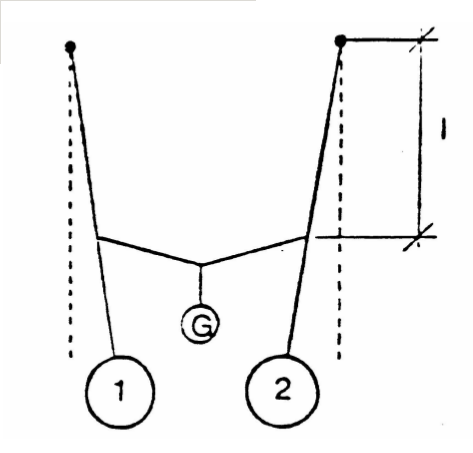
\includegraphics[scale=0.45]{./figure/skizze_kopplung.png}
	\caption{Skizze eines gekoppelten Pendels [1](Abb.7, p.9)}
	\label{fig:gekoppelt_skizze}
\end{figure}
\noindent Die Kopplungslänge \textbf{l} und das Gewicht \textbf{G} beeinflussen die Schwingung des Gesamtsystems. Je nach Anfangsbedingungen kann man drei Sonderfälle unterscheiden:\\
\begin{itemize}
	\item  \textbf{Gleichsinnige Schwingung} \\ beide schwingen parallel mit $\omega_0$, gleicher Phase und gleicher Amplitude
	\item  \textbf{Gegensinnige Schwingung} \\ beide Pendel schwingen mit einer (kopplungsabhängig) höheren Frequenz $\omega_1$, wobei ihre Amplituden gleich sind, sie jedoch einen Phasenversatz von $\phi = \pi$ haben.
	\item  \textbf{Schwebungsfall} \\ zu Beginn schwingt nur ein Pendel mit einer Frequenz $\omega_2$, das zweite ruht. Die gesamte Energie des schwingenden wird langsam auf das ruhende übertragen; dieses beginnt zu schwingen, bis es die ursprüngliche Amplitude des ersten Pendels hat und dieses ruht und der Kreislauf beginnt von vorne.\\
	(der Verlauf der Amplitudenänderung ist periodisch mit $\omega_S$)
\end{itemize}

\noindent Diese Eigenfrequenzen des Systems ergeben sich aus der Lösung der Bewegungsgleichung für gekoppelte Pendel. Es werden 2 Oszillatoren sowie eine zusätzliche Rückstellkraft aus der Kopplung betrachtet.\\
$\omega_S$ und $\omega_2$ lassen sich auch aus den Eigenfrequenzen der gleich- sowie der gegensinnigen Schwingung berechnen:
$$\omega_S = \frac{\omega_1 - \omega_0}{2}$$
$$\omega_2 = \frac{\omega_1 +\omega_0}{2}$$

\noindent Der Kopplungsgrad \textbf{K} ist gegeben durch:
$$K = \frac{\omega_1^2 - \omega_0^2}{\omega_1^2 + \omega_0^2} =  \frac{2\omega_S \omega_2}{\omega_S^2 + \omega_2^2} $$

%%%%%%%%%%%%%%%%%%%%%%%%%%%%%%%%%%%%%%%%%%%%%
% TODO genauer ausformulieren + formeln
%%%%%%%%%%%%%%%%%%%%%%%%%%%%%%%%%%%%%%%%%%%%%

\subsection{Dopplerverschiebung einer bewegten Schallquelle}
Zur Bestimmung der Schallgeschwindigkeit anhand des Dopplereffekts wird in PS1 der Schwebungsfall 2er gekoppelter Oszillatoren (2 Lautsprecher bzw die von ihnen angeregte Luft) verwendet.\\
Der Dopplereffekt ist die Änderung einer Frequenz, wenn die erzeugende Quelle sich relativ zum Beobachter bewegt (klassisches Beispiel: Rettungswagen mit Blaulicht).\\
Anhand der Schwebungsdauer von zwei Schallquellen, die mit gleicher bekannter Frequenz betrieben werden (eine in Bewegung), und der Relativgeschwindigkeit, kann die Schallgeschwindigkeit in Luft durch folgende Relation bestimmt werden:
%$$c_{Luft} = \frac{v}{\frac{\nu}{\nu_0}-1}$$
$$\nu = \nu_0(1 + \frac{v}{c_{Luft}})$$
$\nu_0$ \ldots die Frequenz der Schallquelle\\ 
$\nu$ \ldots die durch den Dopplereffekt veränderte Frequenz\\
$v$ \ldots Bewegungsgeschwindigkeit\\
\\
Die Frequenzverschiebung durch den Dopplereffekt
$$\Delta \nu = \nu_0 - \nu$$
steht im Zusammenhang mit der Schwebungsdauer $T_S$ durch:
$$T_S = \frac{2 \pi}{\Delta \omega}= \frac{1}{\Delta \nu}$$
Durch einsetzen und umformen:
$$\frac{1}{T_S} = \frac{\nu_0}{c_{Luft}}\cdot v$$

Diese lineare Gleichung wird im Versuch benutzt, um aus mehreren Messungen von $T_S$ und $v$ den Anstieg $\frac{\nu_0}{c_{Luft}}$ zu ermitteln und daraus $c$.
%Trägt man $\Delta \nu / \nu_0$ gegen v auf, entspricht der Anstieg der Schallgeschwindigkeit.


\section{Versuchsaufbau:}
\subsection{Drehpendel:}
Als Oszillator, um Dämpfung und Resonanz zu zeigen, wird ein Drehpendel verwendet, hier eine vertikal montierte Kupferscheibe an einer Spiralfeder (Abb. \ref{fig:drehpendel_skizze}).\\
Am Pendel selbst ist ein Zeiger montiert, außen herum eine Scheibe mit einer Skala angebracht, um die relative Amplitude zu messen.\\
Die Dämpfung wird als Wirbelstrombremse realisiert. Daher sind die Angaben der 2 verschiedenen betrachten Dämpfungen in (mA). Die Steuerung der Bremsstärke erfolgt über einen regelbaren Widerstand und ein analoges Amperemeter zum genauen Setup der Dämpfung.\\
Außerdem ist am Versuchsaufbau noch ein Motor montiert, der, zum Messen der Resonanzkurve, als treibende Kraft dient. Seine Drehfrequenz wird durch eine angebrachte Scheibe, mit 10 gleichmäßig verteilten weißen Strichen gemessen, indem mit einem Drehzahlmesser die Zahl ihrer Durchgänge pro Minute bestimmt wird.\\

Zur Messung der Eigenfrequenz und den Werten der Dämpfungskonstanten, werden jeweils Periodendauern mit der Stoppuhr gemessen. Um genauere Ergebnisse zu erhalten wird über mehrere Perioden gemittelt, sowie auch über mehrere Messreihen.\\
Die Dämpfungskonstante (bei 250mA und 350mA Bremsstrom) wird bestimmt, indem mehrere Amplituden im Logarithmus gegen die Zeit aufgetragen werden. der lineare Anstieg ergibt $\delta$.\\
Zur Darstellung der Resonanzkurve werden jeweils, für beide Dämpfungen, die Amplituden für verschiedene Triebfrequenzen (Potentiometer am Motor) aufgetragen und ein Kurvenverlauf mit Splines angenähert.
\begin{figure}[H]
	\centering
	\includegraphics[scale=0.4]{./figure/drehpendel.png}
	\caption{Skizze des Aufbaus des Drehpendels [1](Abb.6, p.7)}
	\label{fig:drehpendel_skizze}
\end{figure}
\subsection{Gekoppeltes Pendel:}

Das hier verwendete gekoppelte Pendel besteht aus 2 Schwerkraftpendel, die mit einem Faden verbunden sind, an dem ein Gewicht befestigt wird (Abb.\ref{fig:gekoppelt_skizze}).\\

Sie werden jeweils per Hand in Schwingung versetzt, um Messungen der Periodendauer (wieder mit Stoppuhr) für die 3 verschiedenen Spezialfälle durchzuführen.\\
Dabei werden jeweils wieder mehrere Periodendauern gemessen und durch ihre Zahldividiert, sowie pro gemessener Eigenfrequenz, Fall und Kopplungsgewicht, mehrere solche Periodendauern bestimmt und über sie gemittelt.\\
Es ist darauf zu achten, dass die Auslenkungen nicht zu groß sind (da ja die Lösungen für ein Schwerkraftpendel mit der Kleinwinkelnäherung erhalten wurden).\\
Aus den 4 Kreisfrequenzen $\omega_0$, $\omega_1$, $\omega_2$ und $\omega_S$ kann pro Kopplungsmasse auf 2 verschiedene Arten der Kopplungsgrad berechnet und anschließend verglichen werden.

\subsection{Dopplerverschiebung einer bewegten Schallquelle:}

Der Dopplereffekt wird in diesem Versuch dargestellt, indem 2 kleine Lautsprecher mit der selben Frequenz betrieben werden (knapp 20kHz, also außerhalb der Hörschwelle eines Erwachsenen), auf die ein Richtmikrophon, verbunden mit einem Oszilloskop, gerichtet ist. Einer der beiden Lautspreche wird, gezogen von einem Motor, auf einer Schiene gleichmäßig auf das Mikrophon zu- oder vom Mikrophon wegbewegt (Abb.\ref{fig:dopplereffekt_skizze})\\
Durch diese Bewegung ergibt sich eine Frequenzverschiebung. In Überlagerung mit dem Signal aus dem stationären Speaker entsteht eine Schwebung, da der Frequenzunterschied nicht sehr groß ist.



\begin{figure}[H]
	\centering
	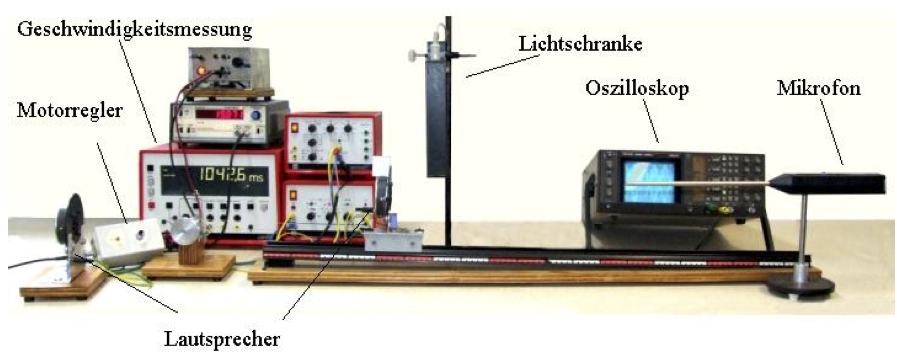
\includegraphics[scale=0.5]{./figure/dopplereffekt_skizze.png}
	\caption{Skizze des Aufbaus für den Dopplereffekt [1](Abb.10, p.14)}
	\label{fig:dopplereffekt_skizze}
\end{figure}

Die Periodendauer der Schwebung wird am Oszilloskop bestimmt. Trotz Umgebungsgeräuschen, lässt sich die Schwebung, vor allem wenn der bewegte Speaker gerade auf gleicher Höhe mit dem unbewegten ist, gut darstellen.\\
Die Geschwindigkeit des bewegten wird mit einer Lichtschranke gemessen, die durch ein am Wagen befestigtes Plättchen unterbrochen und wieder durchgelassen wird. Bei bekannter Breite des Plättchens (3cm) lässt sich so die Geschwindigkeit berechnen.\\
Der Kehrwert der Periodendauer wird gegen die Wagengeschwindigkeiten aufgetragen. Der Lineare Anstieg entspricht der Signalfrequenz $\nu_0$ geteilt durch die Schallgeschwindigkeit in Luft (Raumtemperatur).

\pagebreak
%%%%%%%%%%%%%%%%%%%%%%%%%%%%%%%%%%%%%%%%%%%%%%%%%%%%%%%%%%%%%%%%%%%%%%%
\section{Resultate}
\subsection{Drehpendel}
Bei ausgeschalteter Bremse:\\
$\omega = (3.54 \pm 0.10)$
\begin{figure}[H]
	\centering
	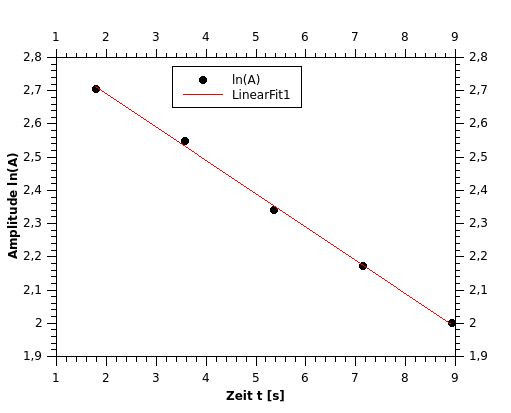
\includegraphics[scale=1.8]{./figure/Messung1_Daempfung_omega0.png}
	\caption{Bestimmung des Dämpfungskoeffizienten (Dämpfung mit 250mA)}
	\label{fig:daempfung_omega0_1}
\end{figure}

\noindent \textbf{Drehpendel - Dämpfung mit 250mA:}\\
Periodendauer (Mittel aus 5 Messungen):\\
$T = (1.7665 \pm 0.013)s$\\
$\Lambda = (-0.1718 \pm 0.0045)s$
$$\delta = \frac{ln(A)}{T} = (0.1003 \pm 0.0024)s^{-1}$$

$$\omega_{0 - 250mA}=(3.558 \pm 0.053)s^{-1}$$
Halbwertsbreite: 3.540 - 3.358:\\
$$\delta_{Halbwertsbreite} = (0.091 \pm 0.010)s^{-1}$$
$$Q_{250mA}=(17.74 \pm 0.50)$$


\end{multicols}
\begin{figure}[H]
	\centering
	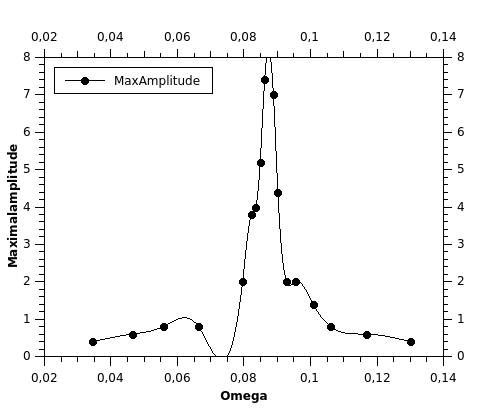
\includegraphics[scale=1.8]{./figure/Messung1_Resonanzkurve_250mA.png}
	\caption{Resonanzkurve (250mA)}
	\label{fig:resonanzkurve_250mA}
\end{figure}


\pagebreak
\begin{multicols}{2}

%\noindent \textbf{Drehpendel - Dämpfung mit 350mA:}\\
\begin{figure}[H]
	\centering
	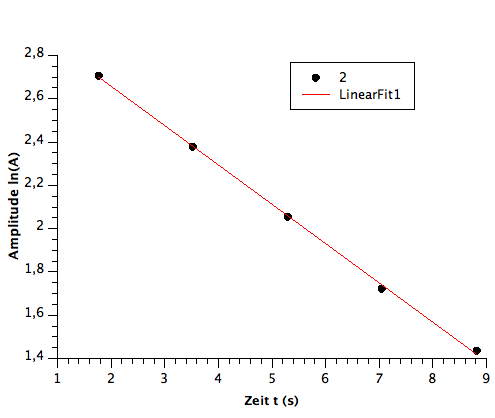
\includegraphics[scale=0.4]{./figure/Messung1_Daempfung_omega0-350mA.png}
	\caption{Bestimmung des Dämpfungskoeffizienten (Dämpfung mit 350mA)}
	\label{fig:daempfung_omega0_350mA}
\end{figure}

\noindent \textbf{Drehpendel - Dämpfung mit 350mA:}\\
\noindent Periodendauer (Mittel aus 5 Messungen):\\
$T = (1.7627 \pm 0.0063)s$\\
$\Lambda = (-0.3203 \pm 0.0048)s$
$$\delta = \frac{ln(A)}{T} = (0.1817 \pm 0.0026)s^{-1}$$

$$\omega_{0 - 350mA}=(3.569 \pm 0.026)s^{-1}$$
Halbwertsbreite: 3.59 - 3.26:\\
$$\delta_{Halbwertsbreite} = (0.165 \pm 0.010)s^{-1}$$
$$Q_{350mA}=(9.82 \pm 0.16)$$

% TODO grafik von Pats QTI 
%\begin{figure}[H]
%	\centering
%	%\includegraphics[scale=0.8]{./figure/Messung2_Daempfung_omega0.png}
%	\caption{Bestimmung des Dämpfungskoeffizienten Dämpfung 2 (350mA)}
%	\label{fig:daempfung_omega0_2}
%\end{figure}

\end{multicols}
\begin{figure}[H]
	\centering
	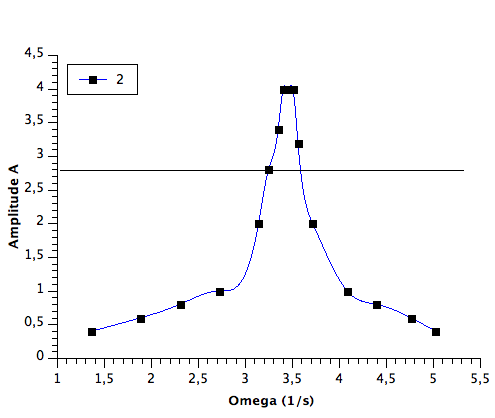
\includegraphics[scale=0.78]{./figure/Messung1_Resonanzkurve_350mA.png}
	\caption{Resonanzkurve (350mA)}
	\label{fig:resonanzkurve_350mA}
\end{figure}


\pagebreak
\begin{multicols}{2}




\subsection{Gekoppelte Pendel}

\noindent Kopplungslänge (beide Massen):\\
$l = (60.5 \pm 0.5 cm)$\\

\noindent Kopplungsmasse 1:\\
$m_1 = (504.3 \pm 0.1)g$

\noindent $\omega_{gk} = \omega_0 = (3.233 \pm 0.020)s^{-1}$\\
$\omega_{geg} = \omega_1 = (3.587\pm 0.034)s^{-1}$\\
$\omega_2 = (3.446 \pm 0.033)s^{-1}$\\
$\omega_{Schwebung}=\omega_S=(0.7276 \pm 0.0082)s^{-1}$

$$K_{\omega_0,\omega_1}=(0.105 \pm 0.012)$$
$$K_{\omega_2,\omega_S}=(0.1044 \pm 0.0026)$$
\\
\\
\noindent Kopplungsmasse 2:\\
$m_2 = (298.0 \pm 0.1)g$

\noindent $\omega_{gk} = \omega_0 = (3.232 \pm 0.018)s^{-1}$\\
$\omega_{geg} = \omega_1 = (3.466\pm 0.028)s^{-1}$\\
$\omega_2 = (3.341 \pm 0.019)s^{-1}$\\
$\omega_{Schwebung}=\omega_S=(0.5076 \pm 0.0026)s^{-1}$

$$K_{\omega_0,\omega_1}=(0.070 \pm 0.011)$$
$$K_{\omega_2,\omega_S}=(0.0754 \pm 0.0096)$$
\\
\\
\subsection{Dopplerverschiebung einer bewegten Schallquelle:}
$\nu_0 = (19590 \pm 10 ) Hz$\\

\noindent Vom Beobachter weg:\\
%B (y-intercept) = 2,169943820978748e-02 +/- 1,351263299960912e-01\\
%A (slope) = 5,036956678235092e+01 +/- 3,421154601278228e+00\\
Steigung: $(50.4\pm 3.5) m^{-1}$\\

\noindent Zum Beobachter hin:\\
%B (y-intercept) = 4,178049407699678e-01 +/- 1,566248245895523e-01\\
%A (slope) = 3,702851334267199e+01 +/- 3,536858402679127e+00\\
Steigung: $(37.0 \pm 3.6) m^{-1}$\\

\noindent Gesamt: $(43.7 \pm 2.6)$
$$c_{Schall} = (448 \pm 27) m/s$$
% \begin{figure}[H]
% 	\centering
% 	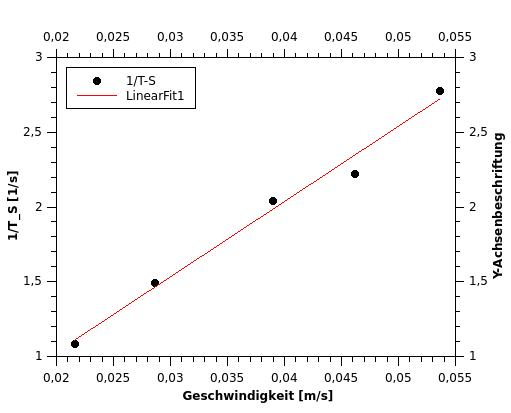
\includegraphics[scale=0.8]{./figure/Aufgabe3_weg_von_Beob.png}
% 	\caption{ Weg von }
% 	\label{fig:weg_von}
% \end{figure}
\end{multicols}
\begin{figure}[H]
	\centering
	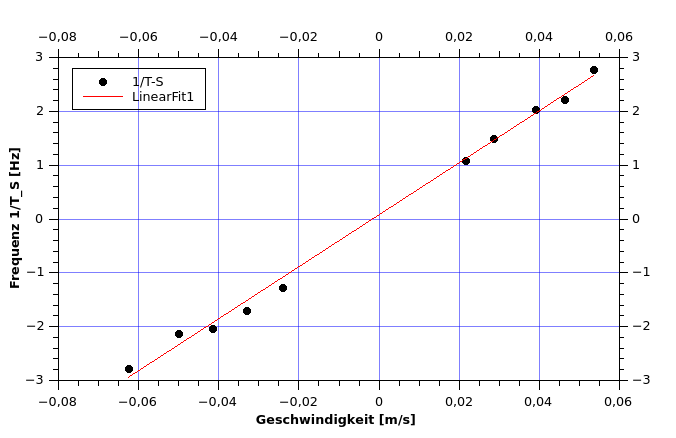
\includegraphics[scale=2.3]{./figure/Dopplereffekt.png}
	\caption{Dopplereffekt lin. Regression mit bewegtem Beobachter in beide Richtungen}
	\label{fig:doppler}
\end{figure}
\begin{multicols}{2}


\pagebreak
%%%%%%%%%%%%%%%%%%%%%%%%%%%%%%%%%%%%%%%%%%%%%%%%%%%%%%%%%%%%%%%%%%%%%%%
\section{Diskussion}
\subsection{Drehpendel}
Die Eigenfrequenz $\omega_0$ unterscheidet sich für beide Dämpfungen kaum von der tatsächlichen Kreisfrequenz $\omega$. Die Dämpfung, die hier einige Perioden zulässt, hat also kaum einen Einfluss auf die Eigenfrequenz.\\

Für beide Dämpfungen wurde die Dämpfungskonstante $\delta$ auf 2 verschiedene Arten bestimmt, nämlich über das Dämpfungsinkrement $\Lambda$, indem der Logarithmus der Amplituden gegen die Schwingungszeit aufgetragen wurde, und als Hälfte der Halbwertsbreite der Resonanzkurve:\\
Vor allem für eine Dämpfung bei 250mA liegen beide gmessenen $\delta$ gut und innerhalb der Unsicherheit, beieinander ($\delta = \frac{ln(A)}{T} = (0.1003 \pm 0.0024)s^{-1}$ und $\delta_{Halbwertsbreite} = (0.091 \pm 0.010)s^{-1}$).\\
Auch für einen Dämpfungsstrom von 350mA ist der Befund plausibel, obwohl hier die Differenz etwas größer ist ($\delta = \frac{ln(A)}{T} = (0.1817 \pm 0.0026)s^{-1}$ und $\delta_{Halbwertsbreite} = (0.165 \pm 0.010)s^{-1}$).\\
Da in dem Versuchsaufbau jedoch einige Abschätzungen eingehen, müsste eine Unsicherheit für ein definitiv angegebenes $\delta$ aus dieser Methode etwas größer abgeschätzt werden:\\
Beispielsweise ist in Abb\ref{fig:resonanzkurve_350mA} gut zu erkennen, dass die Spline-Interpolation genau an der Halbwertsbreite einen Knick macht. Das kann leicht zur Verzerrung führen.\\
Da auch die Frequenzmessung des Motors, sowie seine Einstellmöglichkeit nicht sehr exakt wiederholbar sind, ist die mögliche Schrittweite an Anregfrequenzen eher groß.\\
Wahrscheinlich würde eine gute Wahl der Messpunkte (nicht unbedingt mehr) zu einer besseren Interpolation führen.\\

Auch die Messung der Periodendauer mit Stoppuhr ist natürlich, da menschliche Reaktion der Trigger ist, stark fehleranfällig, wobei hier, durch das Mittel aus mehreren Versuchen, plausible Messergebnisse zu erwarten sind.\\

Die Gütefaktoren $Q_{250mA}=(17.74 \pm 0.50)$ und $Q_{350mA}=(9.82 \pm 0.16)$ unterschieden sich fast um einen Faktor 2. Dies ist schon anschaulich in den Resonanzkurven gut zu erkennen, da die Amplitudenspitze für die stärkere Dämpfung nur etwa die halbe Größe des Peaks bei schwächerer Dämpfung erreicht.\\
Erwartungsgemäß ist also die Resonanz bei schwächerer Dämpfung stärker ausgeprägt (bis sie eben im theoretischen Grenzfall von keiner Dämpfung unendlich scharf wäre).\\


\subsection{Gekoppelte Pendel}
\noindent Für beide Kopplungsgewichte liegen die verschieden berechneten Kopplungsgrade jeweils gut, im Rahmen der Unsicherheit, beieinander.\\
Die Methode der Stoppuhrmessung führt natürlich auch hier zu Verzerrungen, wobei die großen Pendel, montiert vor einer weißen Wand und mit realtiv (zum menschlichen timing) großer Periodendauer, einfache Messungen zulassen.\\
(Die Lichtschranke aus dem Versuch zum Dopplereffekt ließe sich möglicherweise im Weg eines Pendels montieren und würde auch zu noch genaueren Ergebnissen führen, dies ist in diesem Fall jedoch nicht nötig, um die gewünschten Aussagen zu treffen).\\

Der Kopplungsgrad der durch die kleinere Masse erzeugt wird, ist auch geringer.\\
Die Frequenz der gleichsinnigen Schwingung wird erwartungsgemäß kaum von den Kopplungsmassen beeinflusst (schließlich ist hier der Unterschied zwischen beiden schwingenden Gesamt-Systemen nur ein vergleichsweise geringer Massenunterschied von etwa 200g). Auf die anderen Kreisfrequenzen sowie auf die Schwebung, wirken sich die verschiedenen massen jedoch deutlich aus.\\


\subsection{Dopplerverschiebung einer bewegten Schallquelle}
An einem Literaturwert von etwa 340m/s Schallgeschwindigkeit in Luft (Raumtemperatur), ist das Ergebnis dieser Messung mit $c_{Schall} = (448 \pm 27) m/s$ deutlich vorbei.\\
Betrachtet man die beiden Bewegungsrichtungen getrennt, liegt zwar die Messung der Bewegung zum Beobachter hin (1. Quadrant, Abb.\ref{fig:doppler}) etwas näher am Literaturwert, aber auch bei etwa 400m/s.\\
Gut zu erkennen in der Graphik jedenfalls, sind die vom Fit deutlich entfernteren Messpunkte im 3. Quadranten.\\
Die Schwebung ist am Oszilloskop gut erkennbar, es gibt jedoch einen gewissen Ermessensspielraum ihrer Grenzen aufgrund des Hintergrundgrundrauschens (das in diesem Fall tatsächlich dieHintergrundgeräusche des Praktikumsraumes sind).\\
Eine Möglichkeit der Verbesserung, die hier nicht benutzt wurde, ist es, über mehrere Schwebungsperioden zu mitteln.\\

Da der Unterschied zwischen beiden Richtungen sehr deutlich ist, wäre es zwar prinzipiell möglich, dass im Antrieb des Wagens ein systematischer Fehler vorliegt. Nachdem aber für beide Richtungen und der Speaker selbst umgedreht wird, und Motor und Wagen, sowie die Lichtschranke gleich bleiben, ist das eher auszuschließen.\\

Da auch die Gruppe am Vortag Schwierigkeiten hatte, Fehler zu finden, und dennoch sehr ungenaue Ergebnisse bekam, erwarten wir mit einer gewissen Spannung die Durchführung der uns nachfolgenden Gruppe.\\

Ansich ist der Messaufbau sehr klar und alle Messungen durch präzise Messgeräte gestützt. Eine Möglichkeit, genaueres zu erfahren, wäre, den Versuch möglichst spät, wenn Ruhe eingekehrt ist, und für verschieden Frequenzen durchzuführen.


\section{Quellen}
$[1]$ Anleitung, \url{http://www.univie.ac.at/anfpra/neu1/ps/ps1/PS1.pdf}\\
$[2]$ Rohdaten, \url{htts://github.com/blackandcold/Protocols-SS2014-P2/tree/master/PS_1/data}\\

\end{multicols}
\end{document}